%!TEX root = thesis.tex

\begin{tabular}{lll}
\textit{Promotiecommissie} & & \\
& & \\
& & \\
Promotor: 		& Prof. dr. ir. A. W. M. Smeulders 	& Universiteit van Amsterdam\\
& & \\
Co-promotor: 	& Dr. E. Gavves						& Universiteit van Amsterdam\\
& & \\
Overige leden: 	& Prof. dr. C. G. M. Snoek 			& Universiteit van Amsterdam\\
				& Prof. dr. M. Welling 				& Universiteit van Amsterdam \\
				& Prof. dr. M. Shah 				& University of Central Florida \\
				& Dr. P. S. M. Mettes 				& Universiteit van Amsterdam \\

\end{tabular}

\vspace{0.4cm}

\hspace{0.15cm} Faculteit der Natuurwetenschappen, Wiskunde en Informatica

\vfill

\begin{figure}[htb]
\centering

\includegraphics[height=20mm]{chapter_0/UvA_gecentreerd}
\end{figure}

\vspace{15mm}

\noindent
The work described in this thesis has been carried out within the graduate school ASCI, dissertation number \todo{000}, at the Intelligent Sensory Information Systems lab, and the QUVA lab of the University of Amsterdam.

\vspace{5mm}

\begin{figure}[!htb]
\centering
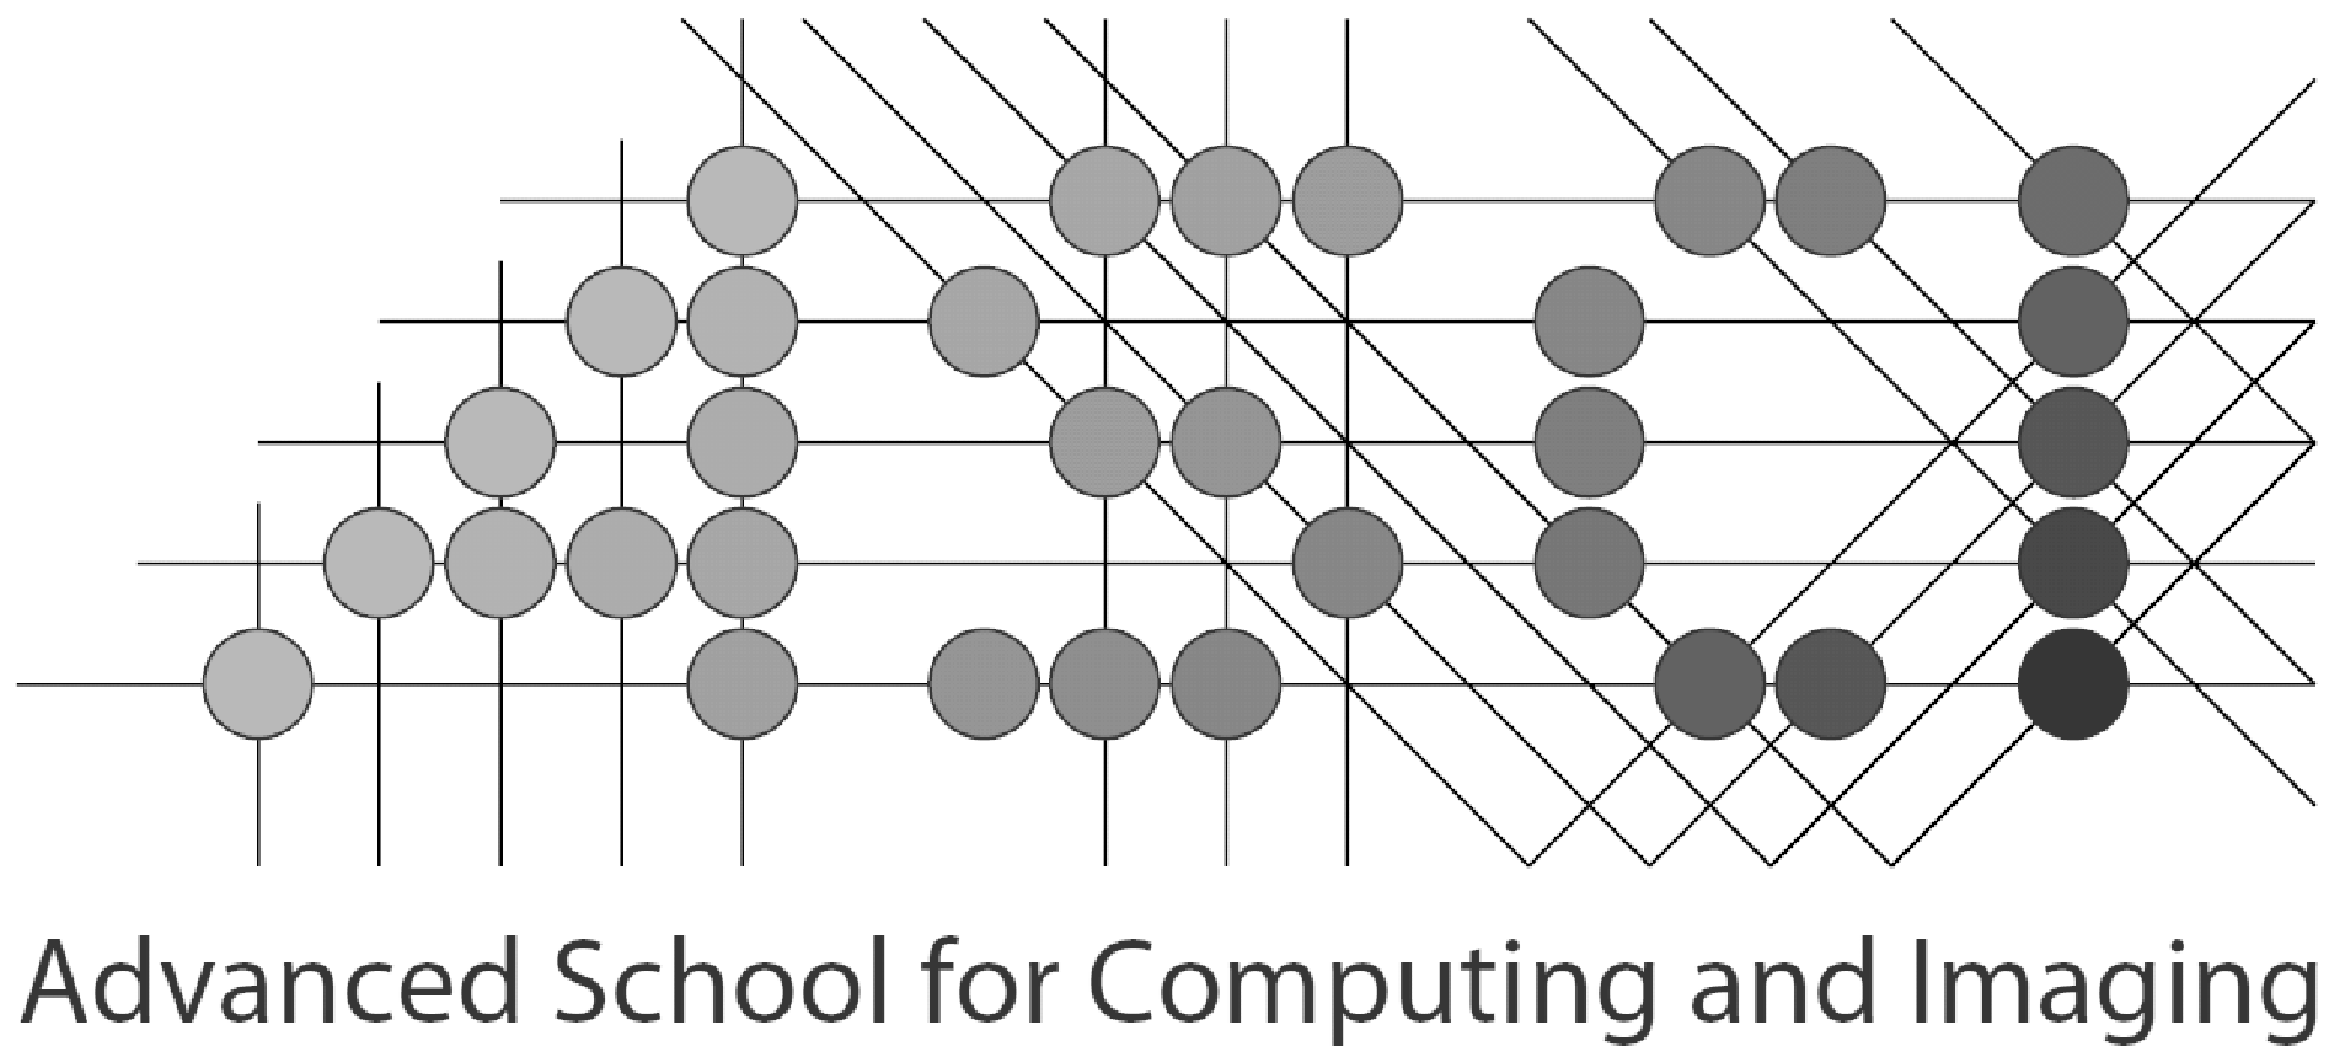
\includegraphics[height=15mm]{chapter_0/ASCIlogo-gray}
\hspace{100pt}

\includegraphics[height=15mm]{chapter_0/quva_logo}
\end{figure}